\documentclass[a4paper,12pt]{article}

\usepackage[utf8]{inputenc}
\usepackage[left=0.5in,right=0.5in,top=1in,bottom=1in]{geometry}
\usepackage{amsmath,amssymb,amsfonts}
\usepackage{pgfplots,graphicx,calc,changepage,caption}
\pgfplotsset{compat=newest}
\usepackage{enumitem}
\usepackage{fancyhdr}
\usepackage[colorlinks = true, linkcolor = blue]{hyperref}

\newcommand{\nats}{\mathbb{N}}
\newcommand{\reals}{\mathbb{R}}
\newcommand{\rats}{\mathbb{Q}}
\newcommand{\ints}{\mathbb{Z}}
\newcommand{\pols}{\mathcal{P}}
\newcommand{\cants}{\Delta\!\!\!\!\Delta}
\newcommand{\eps}{\varepsilon}
\newcommand{\st}{\backepsilon}
\newcommand{\abs}[1]{\left| #1 \right|}
\newcommand{\dom}[1]{\mathrm{dom}\left(#1\right)}
\newcommand{\for}{\text{ for }}
\newcommand{\dd}{\mathrm{d}}
\newcommand{\pd}{\partial}
\newcommand{\spn}{\mathrm{sp}}
\newcommand{\nul}{\mathcal{N}}
\newcommand{\col}{\mathrm{col}}
\newcommand{\rank}{\mathrm{rank}}
\newcommand{\norm}[1]{\lVert #1 \rVert}
\newcommand{\inner}[1]{\left\langle #1 \right\rangle}
\newcommand{\pmat}[1]{\begin{pmatrix} #1 \end{pmatrix}}
\renewcommand{\and}{\text{ and }}
\newcommand{\sech}{\mathrm{sech}}

\newsavebox{\qed}
\newenvironment{proof}[2][$\square$]
    {\setlength{\parskip}{0pt}\par\textit{Proof:} #2\setlength{\parskip}{0.25cm}
        \savebox{\qed}{#1}
        \begin{adjustwidth}{\widthof{Proof:}}{}
    }
    {
        \hfill\usebox{\qed}\end{adjustwidth}
    }

\pagestyle{fancy}
\fancyhead{}
\lhead{Caleb Jacobs}
\chead{APPM 5470: PDEs}
\rhead{Homework \#2}
\cfoot{}
\setlength{\headheight}{35pt}
\setlength{\parskip}{0.25cm}
\setlength{\parindent}{0pt}

\begin{document}
\subsection*{Book Problems:}
\begin{enumerate}[label = \arabic*.]
	\item \textbf{Chapter 3: Problem 3} \\
		Solve for $ u = u(x,t): $
		\[
			u_t + u_x + 3u = e^{2x + t}, \quad u(x,0) = x.
		\]
		
		Using the method of characteristics and with the parameterization
		\[
			\left\langle x(s), t(s), z(s) \right\rangle = \left\langle s, 0, s \right\rangle, \quad s \in \reals,
		\]
		we can obtain a system of ODEs of our PDE as
		\[
			\begin{array}{ccc}
				\frac{\dd t}{\dd \tau} = 1, & \frac{\dd x}{\dd \tau} = 1, & \frac{\dd z}{\dd \tau} =  e^{2x + t} - 3z \\
				t(0) = 0 & x(s) = s & z(s) = s
			\end{array}.
		\]
		Using an integrating factor, we can obtain the solution to this system of ODEs as
		\[
			\begin{array}{ccc}
				t = \tau, & x = \tau + s, & z = \frac{1}{6} \left(e^{2s + 3\tau} - e^{2s - 3\tau}\right) + e^{-3\tau}s
			\end{array}.
		\]
		Next, we can invert $ t $ and $ x $ to obtain our full solution of
		\[
			\begin{array}{ccc}
				\tau = t, & s = x - t, & u(x,t) = z = \frac{1}{6} \left(e^{2x + t} - e^{2x - 5t}\right) + e^{-3t}(x - t)
			\end{array}.
		\]
		Thus, our solution to the PDE above is given by 
		\[
			 u(x,t) = \frac{1}{6} \left(e^{2x + t} - e^{2x - 5t}\right) + e^{-3t}(x - t)\quad \forall\; x,t \in \reals
		\]
    \item \textbf{Chapter 3: Problem 8}
    	\begin{enumerate}[label = (\alph*)]
    		\item Use the method of characteristics to solve the initial value problem
    		\[
    			\begin{cases}
    				u_t + t u_x = u^2, & -\infty < x < \infty, \; 0 < t < 1 \\
    				u(x, 0) = \frac{1}{1 + x^2}, & -\infty < x < \infty
    			\end{cases}.
    		\]
    		
    		Using the method of characteristics with the parameterization 
    		\[
    			\langle x(s), t(s), z(s) \rangle = \left\langle s, 0, \frac{1}{1 + s^2} \right\rangle \quad s \in \reals
    		\]
    		we can obtain the system of ODEs representing the IVP as
    		\[
	    		\begin{array}{ccc}
	    			\frac{\dd t}{\dd \tau} = 1, & \frac{\dd x}{\dd \tau} = t, & \frac{\dd z}{\dd \tau} = z^2 \\
	    			t(0) = 0, & x(0) = s, & z(0) = \frac{1}{1 + s^2}
	    		\end{array}.
    		\]
    		We can solve this system directly to obtain
    		\[
    			\begin{array}{ccc}
    				t = \tau, & x = \frac{1}{2} \tau^2 + s, & z = \frac{1}{1 + s^2 - \tau}
    			\end{array}.
    		\]
    		Then, we can invert $ t $ and $ x $ to obtain the full solution
    		\[
    			\tau = t, \quad s = x - \frac{1}{2} t^2, \quad u(x,t) = z = \frac{1}{1 + \left(x - \frac{1}{2}t^2\right)^2 - t}.
    		\]
    		Thus, our full solution is given by
    		\[
    			u(x,t) = \frac{1}{1 + \left(x - \frac{1}{2}t^2\right)^2 - t} \quad \forall\; x \in \reals \text{ and } t \in [0, 1].
    		\]
    		
    		\item Show that the solution blows up as $ t \to 1 $.
    		
    		To show that solution blows up as $ t \to 1^{-} $, let's first compute the max of $ u(x,t) $ over $ x $. To maximize $ u(x,t) $ for $ x $, we can compute the partial as
    		\[
    			\frac{\dd u}{\dd x} = \frac{2 \left(x - \frac{1}{2}t^2 \right)}{1 + \left(x - \frac{1}{2}t^2\right)^2 - t}.
    		\]
    		Then, a maxima along $ x $ is given when the above derivative is zero (numerator is zero) which happens at
    		\[
    			x = \frac{1}{2}t^2.
    		\]
    		Now plugging $ x = \frac{1}{2}t^2 $ into $ u(x,t) $ yields
    		\[
    			\max_x u(x,t) = u(\frac{1}{2}t^2, t) = \frac{1}{1 + \left(\frac{1}{2}t^2 - \frac{1}{2}t^2 \right)^2 - t} = \frac{1}{1 - t}.
    		\]
    		Finally, taking the limit of this max as $ t \to 1^{-} $ yields
    		\[
    			\lim_{t \to 1^-} \max_x u(x,t) = \lim_{t \to 1^-} \frac{1}{1 - t} = \infty.
    		\]
    		Thus, $ u(x,t) $ blows up as $ t \to 1 $.
    	\end{enumerate}
\end{enumerate}

\subsection*{Additional Problems:}
	\begin{enumerate}[label = \arabic*.]
		\item Solve the given Cauchy problems using the method of characteristics. State and sketch the characteristics and determine the values of $ x $ and $ y $ for which the solution exists.
		\begin{enumerate}[label = (\alph*)]
			\item Solve
			\[
				\begin{cases}
					x u_x + (x + y)u_y = 1, \\
					u(1,y) = y, & y \in [0,1]
				\end{cases}.
			\]
			
			Using the method of characteristics with the parameterization
			\[
				\langle x(s), y(s), z(s) \rangle = \langle 1, s, s \rangle, \quad s \in [0,1]
			\]
			we can obtain the system of ODEs as
			\[
				\begin{array}{ccc}
					\frac{\dd x}{\dd \tau} = x, & \frac{\dd y}{\dd \tau} = x + y, & \frac{\dd z}{\dd \tau} = 1 \\
					x(0) = 1, & y(0) = s, & z(0) = s
				\end{array}.
			\]
			This system can be solved with an integrating factor of $ e^{-t} $ to get the solution
			\[
				x = e^\tau, \quad y = e^\tau (s + \tau), \quad z = s + \tau.
			\]
			Then, inverting $ x $ and $ y $ to get our complete solution yields
			\[
				\tau = \ln(x), \quad s = \frac{y}{x} - \ln(x), \quad u(x,t) = z = \frac{y}{x} \quad x > 0.
			\]
			So, our solution is given by $ u(x, t) = \frac{y}{x} $ with $ x > 0 $, and the characteristics are given by
			\[
				x = e^\tau, \quad y = e^\tau (s + \tau) \quad s \in [0, 1], t \in \reals.
			\]
			A plot of the characteristics is given in Figure \ref{fig:char1}.
			
			\begin{figure}[h!]
				\centering
				\captionsetup{width = 0.8\linewidth}
				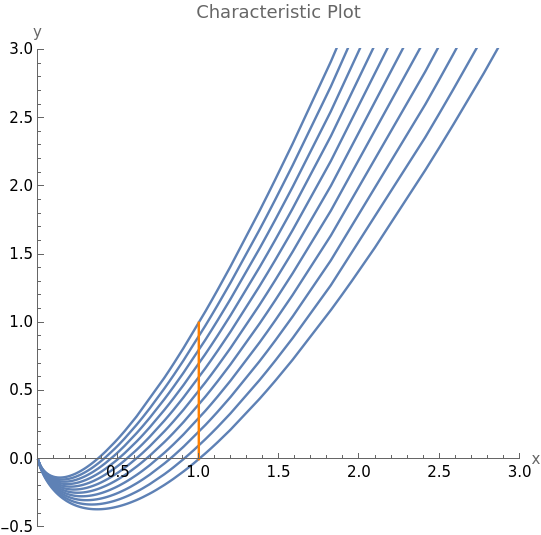
\includegraphics[width = 0.4\textwidth]{images/char1.png}
				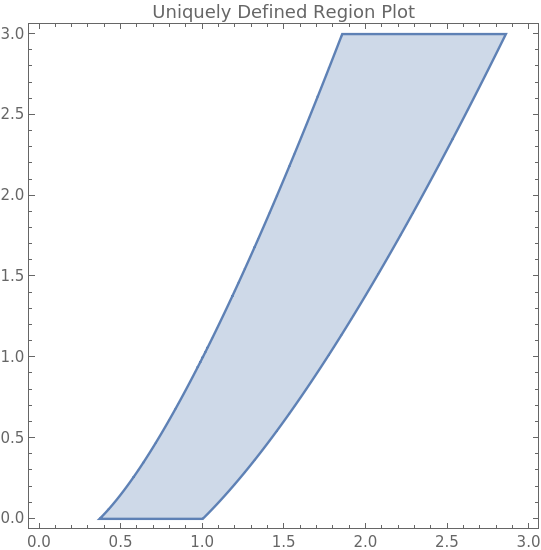
\includegraphics[width = 0.4\textwidth]{images/uniq.png}
				\caption{Left plot of characteristics; blue lines = characteristics; orange line = Cauchy data.
				Right region plot of uniquely defined region; blue region = uniquely defined solution.}
				\label{fig:char1}
			\end{figure}
		
			Furthermore, our solution is uniquely determined when we are on characteristics that originate from the Cauchy data. When we defined our parameterization of the Cauchy data, we had the constraint that $ 0 \leq s \leq 1 $. Taking this constraint and combining with our inverted $ s = \frac{y}{x} - \log(x) $ yields
			\[
				0 < \frac{y}{x} - \log(x) < 1
			\]
			which must defines the region for $ x $ and $ y $ such that $ u(x,y) $ is uniquely determined. The uniquely defined region in the first quadrant can be seen in Figure \ref{fig:char1}
			
			\item Solve 
			\[
				\begin{cases}
					(y + u)u_x + y u_y = x - y \\
					u(x,1) = 1 + x, & x \in \reals
				\end{cases}.
			\]
			
			Using the method of characteristics and the Cauchy data parameterization
			\[
				\langle x(s), y(s), z(s) \rangle = \langle s, 1, 1 + s \rangle \quad s \in \reals
			\]
			we can obtain the system of ODEs modeling our PDE as
			\[
				\begin{array}{ccc}
					\frac{\dd x}{\dd \tau} = y + z, & \frac{\dd y}{\dd \tau} = y, & \frac{\dd z}{\dd \tau} = x - y \\
					x(0) = s, & y(0) = 1, & z(0) = 1 + s
				\end{array}.
			\]
			This system of ODEs is a linear non-homogeneous coupled system of ODEs and so we can solve it using the Lagrange method to obtain the solution
			\[
				x = e^\tau (1 + s) - e^\tau, \quad y = e^\tau, \quad z = e^\tau s + e^{-\tau}.
			\]
			Then, we can invert $ x $ and $ y $ to obtain the explicit solution
			\[
				s = \frac{1}{y^2} + \frac{x}{y} - 1, \quad \tau = \ln(y), \quad u(x,t) = z = \frac{2}{y} - y + x
			\]
			for $ x \in \reals $ and $ y > 0 $. Furthermore, the characteristics are given by
			\[
				x = e^\tau (1 + s) - e^\tau, \quad y = e^\tau \quad \text{ for } s \in \reals, \tau \in \reals.
			\]
			A plot of the characteristics can be seen in Figure \ref{fig:char2}
			
			\begin{figure}[h!]
				\centering
				\captionsetup{width = 0.5\linewidth}
				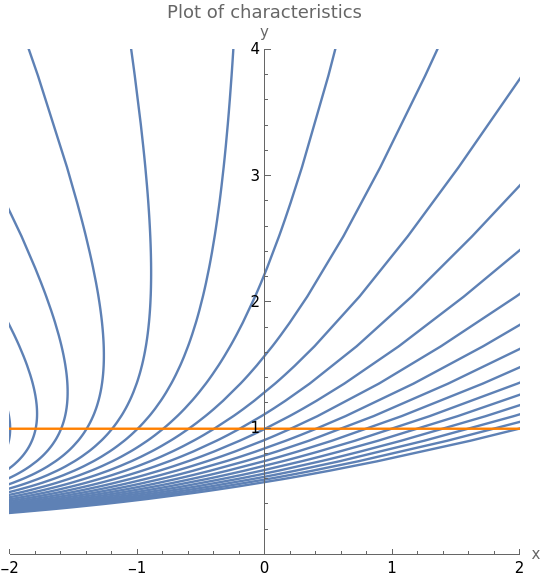
\includegraphics[width = 0.5\textwidth]{images/char2.png}
				\caption{Characteristic curve plot; blue lines = characteristic lines; orange line = Cauchy data}
				 \label{fig:char2}
			\end{figure}
		\end{enumerate}
	
		\item Prove that there exists a $ C^1(\reals) $ solution $ u(x,y) $ to
			\[
				\begin{cases}
					u u_x = u_y = -\frac{1}{2}u, & x \in \reals, y > 0 \\
					u(x,0) = f(x), & x \in \reals
				\end{cases}
			\]
			for $ y \geq 0 $ sufficiently small and $ f \in C^1(\reals) $.
			
			\begin{proof}{}
				First, define
				\begin{align*}
					\vec{x} &= \pmat{x \\ y}, \\
					\vec{a}(\vec{x}) &= \pmat{u \\ 1}, \\
					c(\vec{x}, u) &= - \frac{1}{2}u, \\
					\vec{x}_0(s) &= \pmat{s \\ 1}.
				\end{align*}
				Then, we can define our PDE as
				\[
					\begin{cases}
						\vec{a} \cdot \nabla u = c, & x \in \reals, y > 0 \\
						u(\vec{x}_0) = f(x), & x \in \reals
					\end{cases}.
				\]
				Now, let's compute
				\[
					\det\left[\frac{\pd x_0(s)}{\pd s}, a(\vec{x}_0(s), u_0(s))\right] = 
					\begin{vmatrix}
						\pd_s s & u(s, 0) \\
						\pd_s 0 & 1
					\end{vmatrix}
					=
					\begin{vmatrix}
						1 & u(s, 0) \\
						0 & 1
					\end{vmatrix}
					= 1 - u(s, 0) * 0 = 1 \neq 0.
				\]
				Then, because the calculated determinant is non-zero and $ \vec{x}_0 $ and $ f(x) $ are $ C^1(\reals) $, by Theorem 3.1 of our PDE book by Shearer and Levy, for $ y $ sufficiently small, there exists a $ C^1(\reals) $ function $ u $ that solves our PDE.
			\end{proof}
		
		\item Consider the IBVP
			\[
				\begin{cases}
					u_t + (x + 1)^2 u_x = x, & x > 0, t > 0 \\
					u(x,0) = f(x), & x > 0 \\
					u(0, t) = g(t), & t > 0
				\end{cases}.
			\]
			\begin{enumerate}[label = (\alph*)]
				\item Solve the IBVP using the method of characteristics.
				
				In order to solve this IBVP using the method of characteristics, we need to break our Cauchy data into two surfaces $ \Gamma_1 $ and $ \Gamma_2 $. Our parameterization for each surface can be given as
				\begin{align*}
					\Gamma_1: & \langle x, t, z \rangle = \langle s, 0, f(s) \rangle  \quad s > 0, \\
					\Gamma_2: & \langle x, t, z \rangle = \langle 0, s, g(s) \rangle \quad s > 0.
				\end{align*}
				With our parameterizations, let's begin solving for our solution off of $ \Gamma_1 $. To do so, the method of characteristics gives us the following system of ODEs
				\[
					\begin{array}{ccc}
						\frac{\dd x}{\dd \tau} = (x + 1)^2, & \frac{\dd t}{\dd \tau} = 1, & \frac{\dd z}{\dd \tau} = x \\
						x(0) = s, & t(0) = 0, & z(0) = f(s).
					\end{array}
				\]
				Solving this system of ODEs yields the solutions
				\[
					x = \frac{s + \tau + s \tau}{1 - \tau - s \tau}, \quad t = \tau, \quad z = f(s) - \tau - \ln(1 - \tau - s \tau).
				\]
				Then, we can obtain our explicit solution by inverting $ x $ and $ t $ to get 
				\[
					s = \frac{x - t - x t}{1 + t + x t}, \quad \tau = t
				\]
				which gives us a final solution of
				\[
					u(x,t) = z = f\left(\frac{x - t - x t}{1 + t + x t}\right) - t - \ln\left(1 - t - \frac{x - t - x t}{1 + t + x t} t \right)
				\]
				for $ \Gamma_1 $.
				
				Now let's do the same procedure but for $ \Gamma_2 $. First, we will use the method of characteristics to generate our system of ODEs as
				\[
					\begin{array}{ccc}
						\frac{\dd x}{\dd \tau} = (x + 1)^2, & \frac{\dd t}{\dd \tau} = 1, & \frac{\dd z}{\dd \tau} = x \\
						x(0) = 0, & t(0) = s, & z(0) = g(s).
					\end{array}
				\]
				Then, solving this system of ODEs yields the solutions
				\[
					x = \frac{\tau}{1 - \tau}, \quad t = s + \tau, \quad z = g(s) - \tau + \ln\left(\frac{1}{1 - \tau}\right).
				\]
				Finally, we can find an explicit solution by inverting $ x $ and $ t $ to get
				\[
					s = \frac{t + tx - x}{1 + x}, \quad \tau = \frac{x}{1 + x}
				\]
				which gives us the explicit solution
				\[
					u(x,t) = z = g\left(\frac{t + tx - x}{1 + x}\right) - \frac{x}{1 + x} - \ln\left(1 - \frac{x}{1 + x}\right)
				\]
				for $ \Gamma_2 $. Now, we need to piece our function together. To do so, we need to find a condition that tells us when use one solution over the other. We can find this condition by realizing that both of our Cauchy data curves coincide when $ s = 0 $. Thus, the characteristics that propagate off our curves at $ s = 0 $ will define the line between each solution. So let's pick our characteristic from $ \Gamma_2 $ and set $ s = 0 $ as
				\[
					0 = \frac{t + t x - x}{1 + x}
				\]
				which implies
				\[
					t = \frac{x}{1 + x}.
				\]
				This relation marks the boundary between each solution and so we can write the full explicit solution to our PDE as 
				\[
					u(x,t) =
					\begin{cases}
						f\left(\frac{x - t - x t}{1 + t + x t}\right) - t - \ln\left(1 - t - \frac{x - t - x t}{1 + t + x t} t\right), & t \leq \frac{x}{1 + x} \\
						g\left(\frac{t + tx - x}{1 + x}\right) - \frac{x}{1 + x} - \ln\left(1 - \frac{x}{1 + x}\right), & t > \frac{x}{1 + x}
					\end{cases}.
				\]
				
				\item State conditions on $ f(x) $ and $ g(t) $ such that the solution $ u(x,t) $ is continuous and differentiable.
				
				To have continuity, both regions must have the same function values along $ t = \frac{x}{1 + x} $. So let's evaluate $ u(x,t) $ along this curve (using Mathematica to simplify as we go ):
				\begin{align*}
					\Gamma_1: & u\left(x,\frac{x}{1 + x}\right) = f(0) - \frac{x}{1 + x} - \ln\left(1 - \frac{x}{1 + x}\right) \\
					\Gamma_2: & u\left(x,\frac{x}{1 + x}\right) = g(0) - \frac{x}{1 + x} - \ln\left(1 - \frac{x}{1 + x}\right).
				\end{align*}
				Then, equating our two functions yields the continuity condition
				\[
					f(0) = g(0)
				\]
				which makes sense because we want the characteristics propagating from $ s = 0 $ to be the same along both solutions which also implies that $ f(0) = g(0) $.
				
				Now, to have differentiablity, we need each partial derivative to be the same across $ t = \frac{x}{1 + x} $. The derivatives along $ t = \frac{x}{1 + x} $ are given as follows (Mathematica was used to simplify the expressions)
				\begin{align*}
					\Gamma_1: & \begin{cases}
						u_x\left(x, \frac{x}{1 + x}\right) = \frac{x + f'(0)}{(1 + x)^2} \\
						u_t\left(x, \frac{x}{1 + x}\right) = -f'(0) \\
					\end{cases} \\
					\Gamma_2: & \begin{cases}
						u_x\left(x, \frac{x}{1 + x}\right) = \frac{x - g'(0)}{(1 + x)^2} \\
						u_t\left(x, \frac{x}{1 + x}\right) = g'(0) \\
					\end{cases}
				\end{align*}
				Then, equation our derivatives yields the two relationships
				\[
					\frac{x+f'(0)}{(1 + x)^2} = \frac{x-g'(0)}{(1 + x)^2}
				\]
				and
				\[
					-f'(0) = g'(0).
				\]
				Solving these relations actually produces the same exact constraint which implies that to have differentiablity of $ u(x,t) $, we need
				\[
					f'(0) = -g'(0).
				\]
			\end{enumerate}
		
		\item Consider the IVP for the inviscid Burgers' equation
			\[
				\begin{cases}
					u_t + u u_x = 0, & x \in \reals, t > 0 \\
					u(x,0) = f(x), & x \in \reals
				\end{cases}.
			\]
			\begin{enumerate}[label = (\alph*)]
				\item Suppose $ f(x) = 1 + \tanh(x) $. For what values of $ t > 0 $ does the solution of the IVP remain smooth and single valued? 
				
				To understand when our solution might encounter gradient catastrophe, we need to look at the first derivative of $ f(x) $. In this case, we have
				\[
					f'(x) = \sech^2(x).
				\]
				In this case, we can see that $ f'(x) $ is strictly positive which means $ f(x) $ is monotonically increasing. Then, because $ f(x) $ is increasing, the characteristics continuously fan out for all $ x $ and $ t $ and so our function will remain smooth and single valued for all $ t > 0 $. This can be seen in the characteristic plot of $ f(x) $ in Figure \ref{fig:char4}
				\begin{figure}[h!]
					\centering
					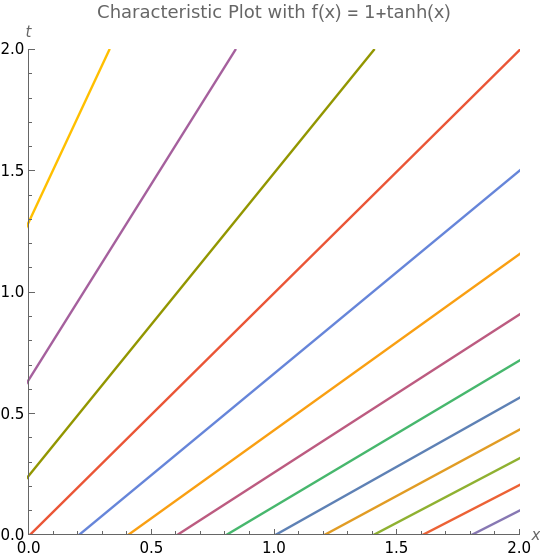
\includegraphics[width = 0.4\textwidth]{images/char4a.png}
					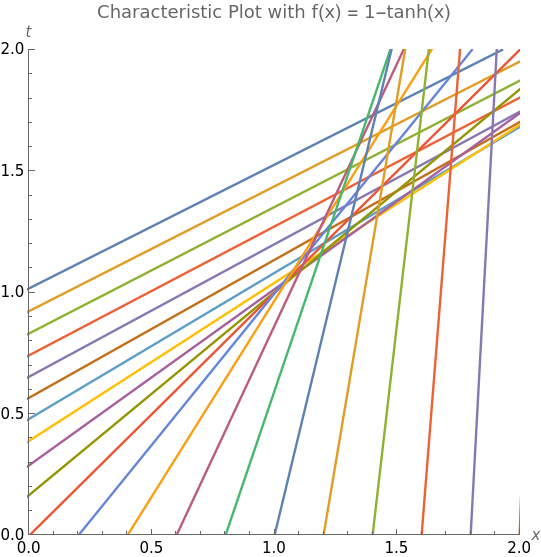
\includegraphics[width = 0.4\textwidth]{images/char4b.png}
					\captionsetup{width = 0.7\textwidth}
					\caption{Characteristic plot of the inviscid Burgers' equation; left has $ f(x) = 1 + \tanh(x) $; right has $ 1 - \tanh(x) $.}
					\label{fig:char4}
				\end{figure}
				
				\item Suppose $ f(x) = 1 - \tanh(x) $. For what values of $ t > 0 $ does the solution of the IVP remain smooth and single valued? 
				
				Just as before, we need to consider the derivative of $ f(x) $ which is given by 
				\[
					f'(x) = -\sech^2(x).
				\]
				Opposite to part (a), now $ f(x) $ is monotonically decreasing. This means that the earliest the characteristics will cross for $ t > 0 $ will be at
				\[
					t_b = - \frac{1}{\min\limits_{x \in \reals} f'(x)} = \frac{1}{\min\limits_{x \in \reals} \sech^2(x)} = \frac{1}{1} = 1.
				\]
				Thus, our solution will be smooth and single valued for $ 0 < t < 1 $. At $ t = t_b = 1$, we will encounter gradient catastrophe which cause the solution to become multivalued. This gradient catastrophe can be seen in Figure \ref{fig:char4} with the crossing of the characteristics starting at $ t = 1 $. Going one step further, we can see that the gradient catastrophe occurs along $ x = t $ at $ t = 1 $ which is the characteristic evolving from the inflection point of $ f(x) $. So, we have
				\[
					(x_b, t_b, u_b) = (1, 1, 1).
				\]
				
				\item Suppose 
					\[
						f(x) =
						\begin{cases}
							0, & x < 0 \\
							x, & 0 \leq x < 1, \quad x \in \reals \\
							1, & 1 \leq x
						\end{cases}
					\]
					
					We can solve this PDE by using the general implicit solution to the inviscid Burgers' equation which is given by
					\[
						u(x,t) = f(x - u(x,t) t).
					\]
					Applying this implicit solution to our piecewise defined $ f $, yields
					\[
						u(x,t) = \begin{cases}
							0, & x - u(x,t) t < 0 \\
							x - u(x,t) t, & 0 \leq x - u(x,t) t < 1 \\
							1, & 1 \leq x - u(x,t) t)
						\end{cases} = \begin{cases}
							0, & x < 0 \\
							\frac{x}{1 + t}, & 0 \leq x < 1 + t\\
							1, & 1 + t \leq x
						\end{cases}.
					\]
					Furthermore, we can see the characteristics in our solution in Figure \ref{fig:char5}. In Figure \ref{fig:char5}, we can see that the characteristics are completely vertical for $ x \leq 0 $ and then they start to transition to have a slope of $ 1 $ by the time we get to $ x = 1 $ and $ t = 0 $. After the characteristics transition to a slope of $ 1 $, they maintain a slope of $ 1 $ as $ x $ increases from $ x = 1 $. All of this is reflected directly in the solution!
					\begin{figure}[h!]
						\centering
						\captionsetup{width = 0.5\textwidth}
						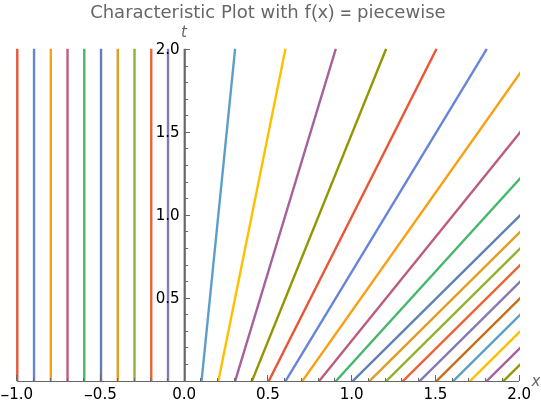
\includegraphics[width = 0.5\textwidth]{images/char4c.png}
						\caption{Characteristic plot with piecewise defined $ f(x) $.}
						\label{fig:char5}
					\end{figure}
			\end{enumerate}
		
		\newpage
		\item Consider the IVP for the wave equation
			\[
				\begin{cases}
					u_{tt} - u_{xx} = 0, & x \in \reals, \quad t > 0\\
					u(x,0) = 0, & x \in \reals \\
					u_t(x,0) = \begin{cases}
						1, & \abs{x} < a \\
						0, & \text{otherwise}
					\end{cases} &
					x \in \reals
				\end{cases}.
			\]
			
			\begin{enumerate}[label = (\alph*)]
				\item Sketch the string profile $ u(x,t) $ at each of the successive instants $ t \in \{a/2, a, 3a/2, 2a, 5a\} $.
				
				To get an idea of what the different string profiles will look like let's use d'Alembert's equation to write out our solution as
				\begin{align*}
					u(x,t) &= \frac{1}{2}(f(x + ct) + f(x - ct)) + \frac{1}{2c} \int_{x - ct}^{x + ct} g(y) \dd y \\
					&= \frac{1}{2}\int_{x - t}^{x + t} \begin{cases}
						1, & \abs{y} < a \\
						0, & \text{otherwise}
					\end{cases} \dd y.
				\end{align*}
				This integral is a little tedious to evaluate and Mathematica would be able to plot it as is but with a little manual effort, I was able to work out a nested piecewise solution of
				\[
					u(x,t) = 
						\begin{cases}
							\begin{cases}
								0, & x + t < -a \\
								\frac{1}{2}(t + x + a), & x - t < -a < x + t \\
								t, & -a < x - t \text{ and } x + t < a \\
								\frac{1}{2}(t - x + a), & x - t < a < x + t \\
								0, & a < x - t
							\end{cases}, & 0 \leq t < a \\
							\begin{cases}
								0, & x + t < -a \\
								\frac{1}{2}(t + x + a), & -a < x + t < a \\
								a, & x - t < -a \text{ and } a < x + t \\
								\frac{1}{2}(t - x + a), & -a < x - t < a \\
								0, & a < x - t
							\end{cases}, & a \leq t
						\end{cases}
				\]
				A plot of the evolving solution can be seen in Figure \ref{fig:string}.
				\begin{figure}[h!]
					\centering
					\captionsetup{width = 0.7\textwidth}
					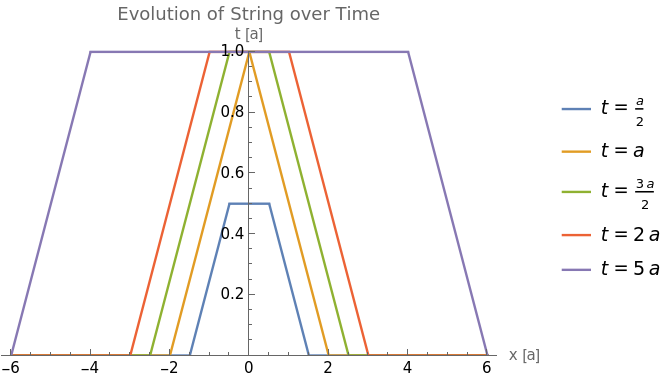
\includegraphics[width = 0.7\textwidth]{images/string.png}
					\caption{Evolution plot of wave equation solution; position and time axis given in terms of $ a $}
					\label{fig:string}
				\end{figure}
				
				\item Find the greatest displacement experienced by the string $ \max_x u(x,t) $ as a function of t.
				
				Looking at our nested piecewise solution and the plot, we can see that the maximum displacement is given by the two middle intervals which can be expressed as
				\[
					\max_x u(x,t) = 
						\begin{cases}
							t, & 0 \leq t < a \\
							a, & a \leq t
						\end{cases}.
				\]
			\end{enumerate}
	\end{enumerate}	
\end{document}